% diffuse/intro.tex          pdflatex ZhCvGo15

% Predrag                                3dec2015
% Tingnan                                2nov2015
% Predrag initial draft                 21nov2014
%         extracted from ChaosBook.org
% \Chapter{diffusion}{2apr2014}{Deterministic diffusion}

% \section{Introduction}

The advances in the theory of dynamical systems have brought a new life
to Boltzmann's mechanical formulation of statistical mechanics,
especially for systems near or far from equilibrium, and yielded new sets
of microscopic dynamics formulas for macroscopic observables such as the
transport coefficients. Sinai, Ruelle and Bowen (SRB) have generalized
Boltzmann's notion of ergodicity for a constant energy surface for a
Hamiltonian system in equilibrium to dissipative systems in
{nonequilibrium} stationary states\rf{sinai,Rue76,bowen}. In this more
general setting the attractor plays the role of a constant energy
surface, and the SRB measure is a generalization of the Liouville
measure. Such measures are purely microscopic and indifferent to whether
the system is at equilibrium, close to equilibrium or far from it. ``Far
for equilibrium'' in this context refers to systems with large deviations
from Maxwell's equilibrium velocity distribution. Furthermore, the theory
of dynamical systems has yielded new sets of microscopic dynamics
formulas for macroscopic observables such as diffusion constants, to
which we turn now.

The classical Boltzmann equation for evolution of 1-particle density is
based on stosszahlansatz, neglect of particle correlations prior to, or
after a 2-particle collision. It is a very good approximate description
of dilute gas dynamics, but a difficult starting point for inclusion of
systematic corrections. In the \po\ theory of deterministic diffusion,
introduced in \refrefs{art91,LorentzDiff,CGS92}, no correlations are
neglected - they are all included in the exact cycle expansions for
transport coefficients such as the diffusion constant.

The Lorentz gas\rf{Lorentz1905} is one of the simplest dynamical
systems of deterministic diffusion. The $2$\dmn\ Lorentz gas is an
infinite scatterer array in which diffusion of a light molecule in a gas
of heavy scatterers is modeled by the motion of a point particle in a
plane bouncing elastically off an array of reflecting disks. The Lorentz
gas is called ``gas'' because one can equivalently think of it as
consisting of any number of point-like fast ``light molecules''
interacting only with the stationary ``heavy molecules'' and not among
themselves.  As the scatterer array is built up from defocusing surfaces,
it is a pure hyperbolic system, and one of the simplest Hamiltonian
dynamical systems that exhibits chaos and deterministic diffusion,
\reffig{fig-chaoticBouncing}.

The original Lorentz gas\rf{Lorentz1905} assumed a random distribution of
heavy scatterers; for such gas a statistical description is unavoidable.
Ergodic properties of a periodic Lorenz gas were first studied by
Sinai\rf{Sinai70}, and its diffusive properties have been extensively
studied ever since%
\rf{Gallavotti75,BunSin80,BunSin81,MacZwa83,Bunimovich85,GasNic90,BuSiCh90}.
For a recent review  see Dettmann\rf{Dettm14}.

\begin{figure}[htbp]
	\begin{center}
		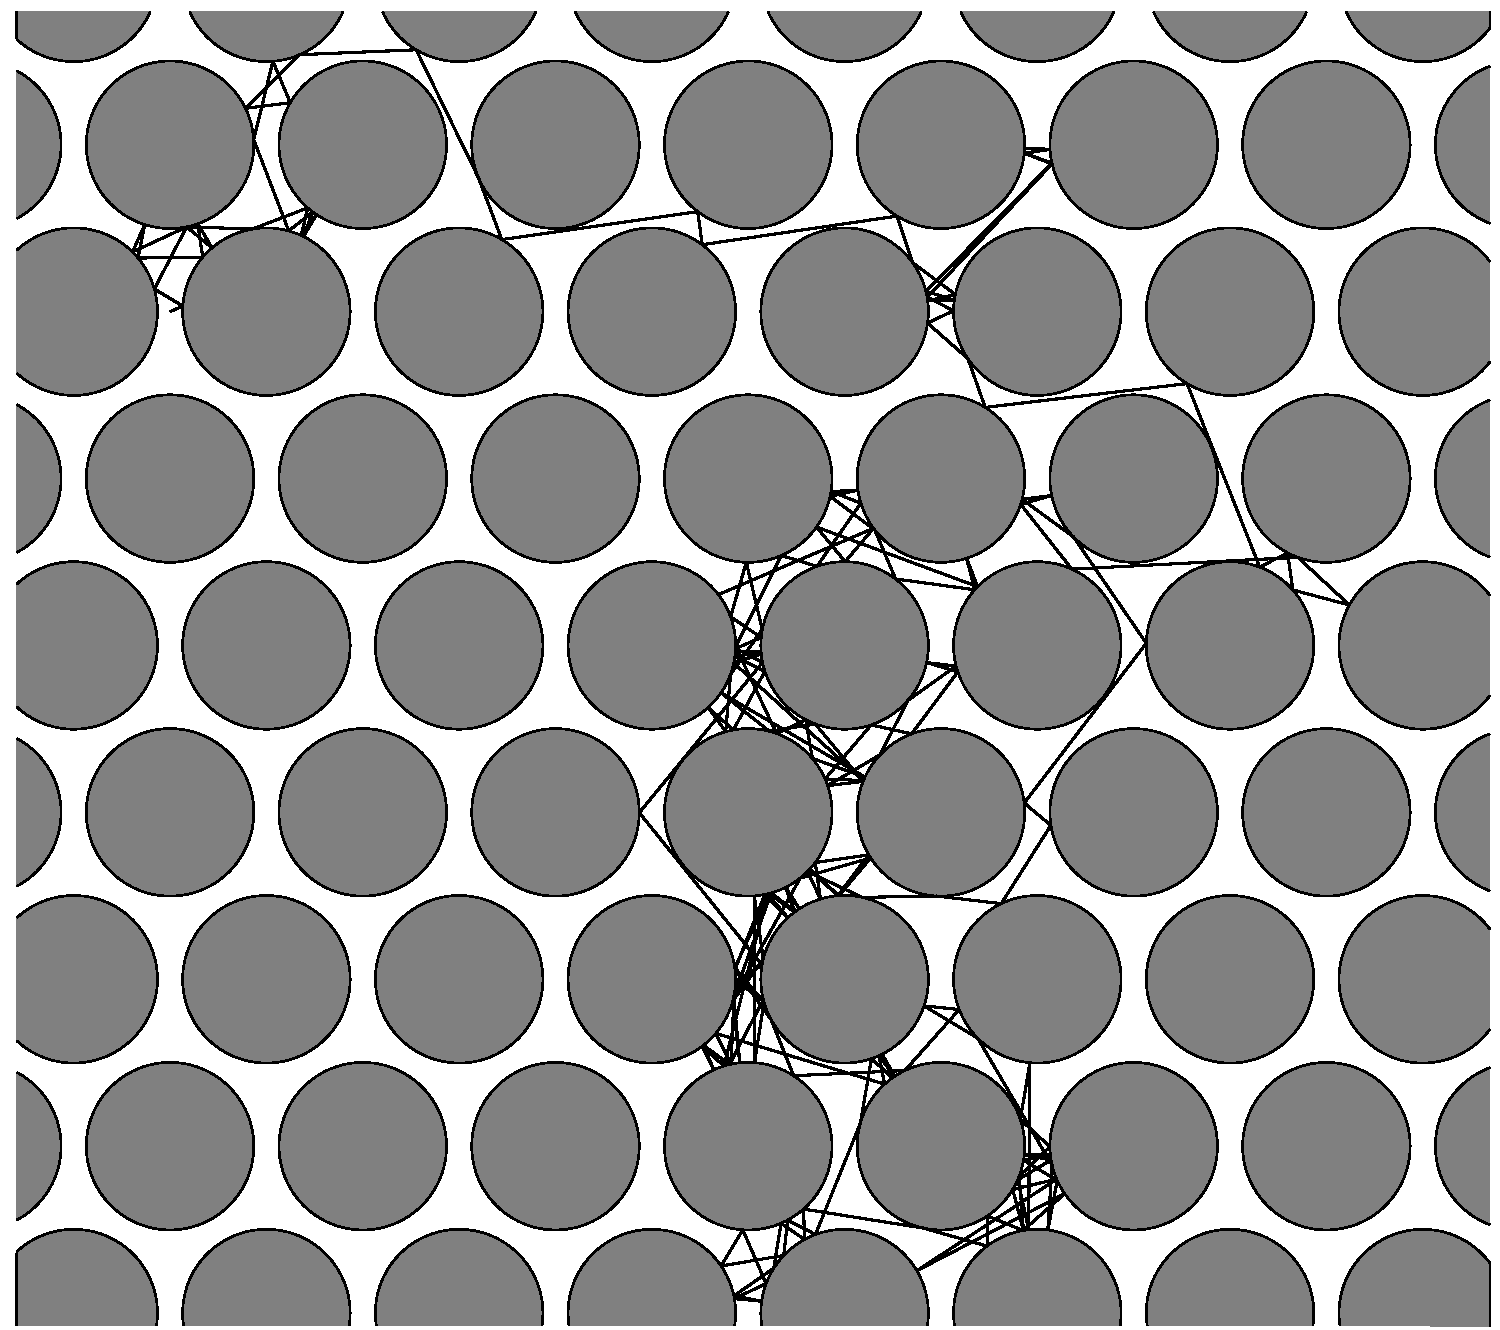
\includegraphics[width=0.45\textwidth]{diffuseChaoticBouncing}
	\end{center}
	\caption[]{\label{fig-chaoticBouncing}
		A chaotic trajectory of a finite horizon Lorentz gas
		point particle bouncing in a
		hexagonal array of disks. The disks are spaced closely enough
		so that the no free flight segment is of infinite length.
	}
\end{figure}
\PC{2015-10-21} {make our own \reffig{fig-chaoticBouncing}\,(a), otherwise
	we have to ask J.-P. Eckmann for permission to use it. It has not been
	published. Similarly, we need our own \reffig{fig-chaoticBouncing}\,(b),
	I do not remember where this one is from.}

The approach introduced in \refref{LorentzDiff} and tested in
\refref{CGS92}, exploits the fact that the periodic Lorentz gas can be
constructed by putting together translated copies of an elementary cell.
Therefore quantities characterizing global dynamics, such as the Lyapunov
exponent and the diffusion constant, can be computed from the dynamics
restricted to the elementary cell.

In \refref{LorentzDiff} some effort, unsuccessful, was made to derive a diffusion
formula for the fully symmetry-reduced dynamics, involving only
quantities computed within the fundamental domain. The fact that lattice
translations do not commute with the symmetry group within the elementary
cell makes this apparently a difficult task. The main achievement of this paper is
a new proposal how to extend \po\ theory in order to solve this
vexing problem.

To investigate the transport property of such systems, we apply cycle
expansions\rf{DasBuch} to the analysis of {\em diffusion coefficient}.
The resulting formulas are exact; no probabilistic assumptions are made,
and all correlations are taken into account by the  inclusion of cycles
of all periods. While existing cycle expansion theory yields the correct
result by tiling the {\statesp} into elementary cells, the convergence
rate is slow because of bad shadowing and poor choice of symbolic
grammar\rf{CGS92}. In this paper we propose a novel approach that
significantly improves the efficiency of cycle expansion formula, by
factorizing the non-commuting rotational and translational symmetry and
using periodic orbits in the fundamental domain.

% The infinite extent systems for which the  periodic orbit theory yields
% formulas for diffusion and other transport  coefficients are spatially
% periodic, the global {\statesp} being tiled with  copies of a elementary
% cell.


\bigskip
=========== TO REUSE ========


\bigskip

    \PC{2015-10-21}
    {the text from Cvitanovi\'c, Gaspard and Schreiber\rf{CGS92}}
This might seem a hopeless task, as one
has to deal with all periodic and aperiodic
solutions of an infinitely extended system. An
approach based on larger and larger finite portions of the system is described
in \refref{GasNic90}, with the diffusion constant related to
%the scaling behaviour of
the escape rates from such finite portions.
%with its size.
%PG
As far as escape rates are obtained in direct numerical simulations
this approach has been shown to be effective\rf{GaBaMaHo92}.
However, from the cyclists point of view
%PG
where the rates are calculated from the periodic orbits,
this approach is impractical; with each added disk new peculiarities arise
in the enumeration of periodic orbits, and with current
methods there is little hope of getting results for more than a few disks,
and no hope of approaching the desired scaling limit.

When this elementary cell is itself invariant under a discrete symmetry
group $G$ the lattice can be tiled into images under $G$ and the lattice
translations of a fundamental domain.

The exact results are sometimes counterintuitive, and might help us
decide whether a diffusive phenomenon whose microscopic dynamics is hard
to observe directly, such as conductance fluctuations in a mesoscopic
device, is due to impurities or to deterministic transport. For example,
as some parameter (such as mean free flight time) is increased, the
deterministic diffusion coefficient reveals a non-monotone, fractal
dependence.

In \refsect{s-Lorentz}

In \refsect{s-POT}
we briefly review the formulas for diffusion
coefficients in the $2$\dmn\ periodic Lorentz gas, using dynamics
restricted in elementary cell.
In \refsect{s-fundDiff} we
factorize the rotational symmetry and derive the diffusion coefficient
using fundamental domain cycles.

Because we will work with different
kinds of \statesp s, through out the text we will repeatedly using tildes
($\tilde{\quad}$), nothings and hats ($\hat{\quad}$) atop symbols to
signify the dynamical quantities in the fundamental domain, elementary
cell and full state space, respectively.
